\pagestyle{plain}
\subsection{波动光学}

\begin{enumerate}
	\item[\textbf{11-27}] 用白光照射杨氏双缝,已知$d=1.0\,\mathrm{mm}$,$D=1.0\,\mathrm{m}$,设屏无限大.
	\begin{enumerate}
		\item 求 $\lambda=500\,\mathrm{nm}$ 的第 $4$ 级明条纹位置及明条纹间距;
		\item 求 $\lambda=600\,\mathrm{nm}$ 的光理论上在屏上可呈现的最大级数;
		\item $\lambda=500\,\mathrm{nm}$ 和 $\lambda=600\,\mathrm{nm}$ 的光在屏上什么位置开始发生重叠？
	\end{enumerate}
	
	\vspace{5cm}

	\item[\textbf{11-30}] 在双缝干涉中,波长 $\lambda=550.0\,\mathrm{nm}$ 的单色平行光垂直入射到缝间距 $d=2\times10^{-4}\,\mathrm{m}$ 的双缝上,屏到缝间距 $D=2\,\mathrm{m}$.
	\begin{enumerate}
		\item 求中央明纹两侧的两条第 $10$ 级明条纹中心间距;
		\item 用一厚度 $e=6.6\times10^{-6}\,\mathrm{m}$、折射率 $n=1.58$ 的云母片覆盖一缝后,零级明条纹将移动到原来的第几级明条纹处？
	\end{enumerate}
	
	\vspace{10cm}

	\item[\textbf{11-35}] 如图~\ref{fig:11-35}~所示,波长为 $680.0\,\mathrm{nm}$ 的平行光垂直照射到长为 $L=0.12\,\mathrm{m}$ 的两块玻璃片上,两玻璃片一边相互接触,另一边被直径 $d=0.048\,\mathrm{mm}$ 的细钢丝隔开.
	\begin{enumerate}
		\item 求两玻璃片间的夹角 $\theta$;
		\item 相邻两明条纹间空气薄膜的厚度差是多少？
		\item 相邻两暗条纹的间距是多少？
		\item 在玻璃片上呈现多少条明条纹？
	\end{enumerate}
	
	\begin{figure}[H]
		\centering
		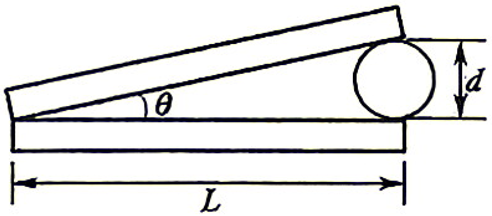
\includegraphics[width=0.3\linewidth]{figures/11-35}
		\caption{习题11-35图}
		\label{fig:11-35}
	\end{figure}
	
	
	\vspace{5cm}

	\item[\textbf{11-43}] 波长 $\lambda=600\,\mathrm{nm}$ 的单色光垂直入射到宽度为 $a=0.01\,\mathrm{mm}$ 的单缝上,观察夫琅禾费衍射图样,透镜焦距 $f=1.0\,\mathrm{m}$,屏幕在透镜的焦平面处,求：
	\begin{enumerate}
		\item 屏上中央明条纹的宽度 $\Delta x_0$ 和半角宽度;
		\item 第二级暗纹所对应的衍射角 $\theta_2$;
		\item 第二级暗纹离透镜焦点的距离 $x_2$.
	\end{enumerate}
	
	\vspace{5cm}

	\item[\textbf{11-44}] 波长为 $680\,\mathrm{nm}$ 的单色可见光垂直入射到缝宽为 $a=1.25\times10^{-4}\,\mathrm{cm}$ 的透射光栅上,观察到第四级谱线缺级.
	\begin{enumerate}
		\item 此光栅每厘米有多少条狭缝？
		\item 求在屏上呈现的光谱线的全部级次和条纹数.
	\end{enumerate}
	
	\vspace{5cm}

	\item[\textbf{11-45}] 设某种波长 $\lambda_1$ 的光与波长 $\lambda_2=486.1\,\mathrm{nm}$ 的光均为平行光,它们同时垂直入射到光栅上.若 $\lambda_1$ 光的第三级光谱线与 $\lambda_2$ 光的第四级光谱线恰好重合在离中央明条纹距离为 $5\,\mathrm{mm}$ 处,设透镜焦距为 $0.50\,\mathrm{m}$.求：
	\begin{enumerate}
		\item $\lambda_1$ 的值;
		\item 光栅常量.
	\end{enumerate}
	
	\vspace{12cm}

	\item[\textbf{11-47}] 波长为 $600\,\mathrm{nm}$ 的单色光垂直入射到一光栅上,第二和第三级明条纹分别出现在 $\sin\theta_2=0.20$ 和 $\sin\theta_3=0.30$ 处,第四级缺级,问：
	\begin{enumerate}
		\item 光栅常量是多少？
		\item 狭缝最小可能宽度有多大？
		\item 按上述选定的 $a$、$b$ 值,实际呈现的全部级次为多少？
	\end{enumerate}
	
	\vspace{5cm}

	\item[\textbf{L11-1}] 很薄的云母片($n=1.58$)覆盖在双缝实验中的一条缝上,如图~\ref{fig:L11-1}~所示,这时屏幕上的零级明条纹移到原来的第 $7$ 级明条纹的位置上.如果入射光波长为 $550\,\mathrm{nm}$,试问此云母片的厚度为多少？
	
	\begin{figure}[H]
		\centering
		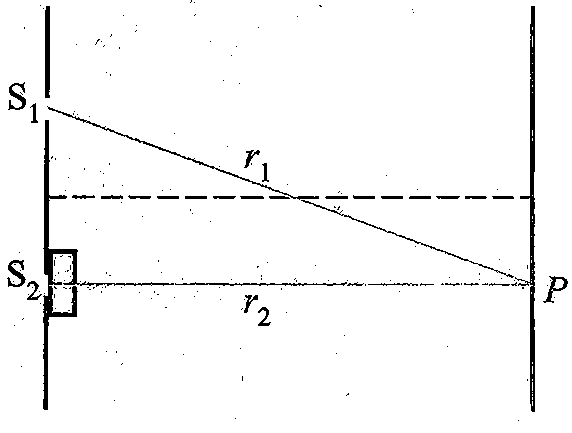
\includegraphics[width=0.25\linewidth]{figures/L11-1}
		\caption{例题11-1图}
		\label{fig:L11-1}
	\end{figure}
	
	
	\vspace{8cm}

	\item[\textbf{L11-2}] 在一光学元件的玻璃(折射率 $n_{3}=1.5$)表面上镀一层厚度为 $e$、折射率为 $n_{2}=1.38$ 的氟化镁薄膜,为了使入射白光中对人眼最敏感的黄绿光($\lambda=550\,\mathrm{nm}$)反射最小,试求薄膜的厚度.
	
	\begin{figure}[H]
		\centering
		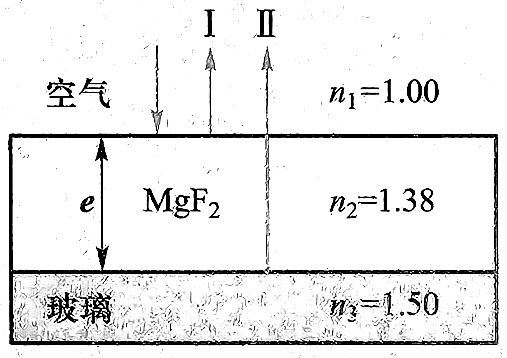
\includegraphics[width=0.3\linewidth]{figures/L11-2}
		\caption{例题11-2图}
		\label{fig:l11-2}
	\end{figure}
	
	
	\vspace{5cm}

	\item[\textbf{L11-5}] 设光栅平面和透镜都与屏幕平行,在透射光栅上每厘米有 $5\,000$ 条刻线,用它来观察钠黄光($\lambda = 589\,\mathrm{nm}$)的光谱线.问：
	
	\begin{enumerate}
		\item 当光线垂直入射到光栅上时,能看到的光谱线的最高级数 $k_m$ 是多少？
		\item 当光线以 $\varphi = 30^\circ$ 的入射角(入射光线与光栅平面的法线的夹角)斜入射到光栅上时,能看到的光谱线的最高级数 $k'_m$ 是多少？
	\end{enumerate}
	
	
	
\end{enumerate}
